\documentclass{patmorin}
\listfiles
\usepackage{pat}
\usepackage{paralist}
\usepackage{dsfont}  % for \mathds{A}
\usepackage[utf8x]{inputenc}
\usepackage{skull}
\usepackage{paralist}
\usepackage{graphicx}
\usepackage[noend]{algorithmic}
\usepackage{bbm}  % needed for \mathbbm{1}
\usepackage{listings}
% \usepackage{xcolor}

\usepackage[normalem]{ulem}
\usepackage{cancel}
%\usepackage{enumitem}

\usepackage{todonotes}


\newcommand{\ipat}[1]{\textcolor{Maroon}{#1}}
\newenvironment{epat}{\color{Maroon}}{}

% etoolbox allows for robust commands that don't need \protect, e.g.
% \newrobustcmd{\onesub}{\mathord{\includegraphics{figs/one-sub}}}
% \subsection{Approximate Voronoi Diagrams in $G^{\onesub}_k$}
\usepackage{etoolbox}

\usepackage[longnamesfirst,numbers,sort&compress]{natbib}

\usepackage[mathlines]{lineno}
\setlength{\linenumbersep}{2em}
% \linenumbers
% \rightlinenumbers
% \linenumbers
\newcommand*\patchAmsMathEnvironmentForLineno[1]{%
 \expandafter\let\csname old#1\expandafter\endcsname\csname #1\endcsname
 \expandafter\let\csname oldend#1\expandafter\endcsname\csname end#1\endcsname
 \renewenvironment{#1}%
    {\linenomath\csname old#1\endcsname}%
    {\csname oldend#1\endcsname\endlinenomath}}%
\newcommand*\patchBothAmsMathEnvironmentsForLineno[1]{%
 \patchAmsMathEnvironmentForLineno{#1}%
 \patchAmsMathEnvironmentForLineno{#1*}}%
\AtBeginDocument{%
\patchBothAmsMathEnvironmentsForLineno{equation}%
\patchBothAmsMathEnvironmentsForLineno{align}%
\patchBothAmsMathEnvironmentsForLineno{flalign}%
\patchBothAmsMathEnvironmentsForLineno{alignat}%
\patchBothAmsMathEnvironmentsForLineno{gather}%
\patchBothAmsMathEnvironmentsForLineno{multline}%
}


% Taken from
% https://tex.stackexchange.com/questions/42726/align-but-show-one-equation-number-at-the-end
\newcommand\numberthis{\addtocounter{equation}{1}\tag{\theequation}}

\definecolor{brightmaroon}{rgb}{0.76, 0.13, 0.28}
\definecolor{linkblue}{rgb}{0, 0.337, 0.227}
\newcommand{\defin}[1]{\emph{\color{brightmaroon}#1}}
\setlength{\parskip}{1ex}

\title{\MakeUppercase{A Universal Geometric Graph for Plane Graphs}\thanks{This research was partly funded by NSERC.}}
\author{Friends from Dagstuhl 24062}

\DeclareMathOperator{\VE}{\mathit{VE}}
\DeclareMathOperator{\sd}{subdist}
\DeclareMathOperator{\len}{len}


\date{}


\begin{document}

\maketitle
\renewcommand{\E}{\mathbb{E}}
\renewcommand{\Pr}{\mathbb{P}}

\begin{abstract}
  We show that there exists a geometric graph $U_n$ having $O(n^3\log n)$ edges with the property that, for any $n$-vertex plane graph $G$ there is an isomorphism from $G$ into a non-crossing subgraph of $U_n$ that preserves the combinatorial embedding of $G$.  In other words, $U_n$ contains a non-crossing straight-line drawing of $G$ as a subgraph.
\end{abstract}

\section{Introduction}



\section{Stuff}

\subsection{Majorizing Sequences}

Define the order $r$ \defin{majorizing sequence} $S_r$ as the sequence of integers:
\[
   S_r := s_{r,1},\ldots,s_{2^{r+1}-1} :=
    \begin{cases}
      1& \text{if $r=0$} \\
      S_{r-1},2^{r+1}-1,S_{r-1} & \text{otherwise}
    \end{cases}
\]
so that, for example, $S_3=1,3,1,7,1,3,1,15,1,3,1,7,1,3,1$.\footnote{The sequence $S_r$ can also be defined by taking a complete binary tree $T_r$ of height $r$ and listing the sizes of subtrees of $T_r$ in the order they are encountered by an in-order traversal of $T_r$.}  It is straightforward to verify that the length of $S_r$ is indeed $n_r:=2^{r+1}-1$ and that the sum of the values in $S_r$ is
\begin{equation}
  \Sigma_r := \sum_{i=1}^{n_r} s_{r,i} = r2^{r+1}+1 \enspace . \label{sigma_r}
\end{equation}
The following well known lemma [CITATION] says that every length-$\ell$ subsequence of $S_r$ contains a value greater than or equal to $\ell$.
\begin{lem}
  For all positive integers $r$, $i\le 2^{r+1}-1$, and $\ell\le 2^{r+1}-i$, $\max\{s_{r,i},\ldots,s_{r,i+\ell-1}\}\ge \ell$.
\end{lem}

\subsection{The Universal Graph}

Let $c$, $r$, and $n$ be positive integers and let $U_{n,r,c}$ be the graph with vertex set
\[
  V(U_{n,r,c}):=\{ u_{i,j}: (i,j)\in\{1,\ldots,2^{r+1}-1\}\times \{1,\ldots,n\}\}
\]
and edge set
\begin{align*}
  E(U_{n,r,c}) & := \left\{ u_{i,j}u_{i',j'} \in V(U_{n,r,c})^2: |i-i'| \le c\max\{s_{r,i},s_{r,i'}\}\right\} \\
  & \quad {}\cup\left\{u_{i,j}u_{i',j}:i,i'\in\{1,\ldots,2^{r+1}-1\}\right\}\enspace .
\end{align*}
In words, each row $u_{1,j},\ldots,u_{2^{r+1}-1,j}$ is a clique and each vertex $u_{i,j}$ is connected to all the vertices in columns $i-cs_{r,i},\ldots,i+cs_{r,i}$.

\ipat{TODO: Double the number of vertices so that each column becomes a set of $2n$ points on a convex curve.}

We treat $U_{n,r,c}$ as a geometric graph by assigning each vertex $u_{i,j}$ an x-coordinate equal to $i$.  The $y$ coordinate of $u_{i,j}$ is equal to some value $y_j$ defined as follows:  $y_1:=0$ and, for $j>1$, $y_j$ is any sufficiently large value such that all points in $u_{1,j},\ldots,u_{2^{r+1}-1,j}$ are above every non-vertical line defined by two points in $\{u_{i',j'}:(i',j')\in\{1,\ldots,2^{r+1}-1\}\times\{1,\ldots,j-1\}\}$.

Our universal graph for $n$-vertex planar graphs is the graph $U_{n,b+\lceil\log_2 n\rceil,c}$ for some constants $b$ and $c$ that will be discussed later.

\subsection{Canonical Orderings and Stingray Decomposition}

A \defin{triangulation} is a plane graph whose faces (including the outer face) are bounded by triangles ($3$-cycles). A \defin{near triangulation} is a plane graph whose outer face is bounded by a cycle and whose interior faces are all triangles.

Let $G$ be a triangulation whose outer face is bounded by a cycle $v_1,v_2,v_n$.  Then, a total ordering $v_1,\ldots,v_n$ of $V(G)$ is a \defin{canonical ordering} if, for each $i\in\{3,\ldots,n\}$,  $G[v_1,\ldots,v_i]$ is a near-triangulation that has $v_i$ on its outer face.


Let $v_1,\ldots,v_n$ be a canonical ordering of $G$. For each $i\in\{1,\ldots,n\}$, let $G_i:=G[v_1,\ldots,v_i]$.  For each $i\in\{3,\ldots,n\}$, the outer face of $G_i$ contains exactly two edges $u_iv_i$ and $v_iw_i$ that are not on in $G_{i-1}$.  For each $i\in\{2,\ldots,n\}$, let $F_i$ be the graph with vertex set $V(F_i):=\{v_1,\ldots,v_i\}$ and edge set $\{v_1v_2\}\cup\bigcup_{j=3}^n\{u_iv_i,v_iw_i\}$.  We treat each $F_i$ as a directed acyclic graph with a single source $v_1$ and a single sink $v_2$ in which the orientation of each edge in $F_i$ is either inherited from $F_{i-1}$ or (if the edge is $u_iv_i$ or $v_iw_i$) chosen to ensure that $F_i$ is acyclic with single source $v_1$ and single sink $v_2$.








Our proof requires a type of canonical ordering, which motivates the following definition. A \defin{stingray} $(x_1,\ldots,x_r)$ in a near-triangulation $G$ is a maximal path $x_1,\ldots,x_r$ on the outer face of $G$ with a special vertex $x_i$ (the \defin{stinger}) that has the following properties (see \cref{crow}):
\begin{compactenum}
  \item $G-\{x_1,\ldots,x_r\}$ is a near-triangulation;
  \item for any $a\in\{1,\ldots,i-1\}$ and $b\in\{i+1,\ldots,r\}$, the vertices $x_a$ and $x_b$ each have degree $2$ in $G-\{x_1,\ldots,x_a,x_b,\ldots,x_r\}$.
\end{compactenum}
Note that the definition of a stingray includes the special case $r=1$ in which the stingray consists of a single vertex $x_1$ such that $G-x_1$ is a near-triangulation.
\begin{figure}
  \begin{center}
    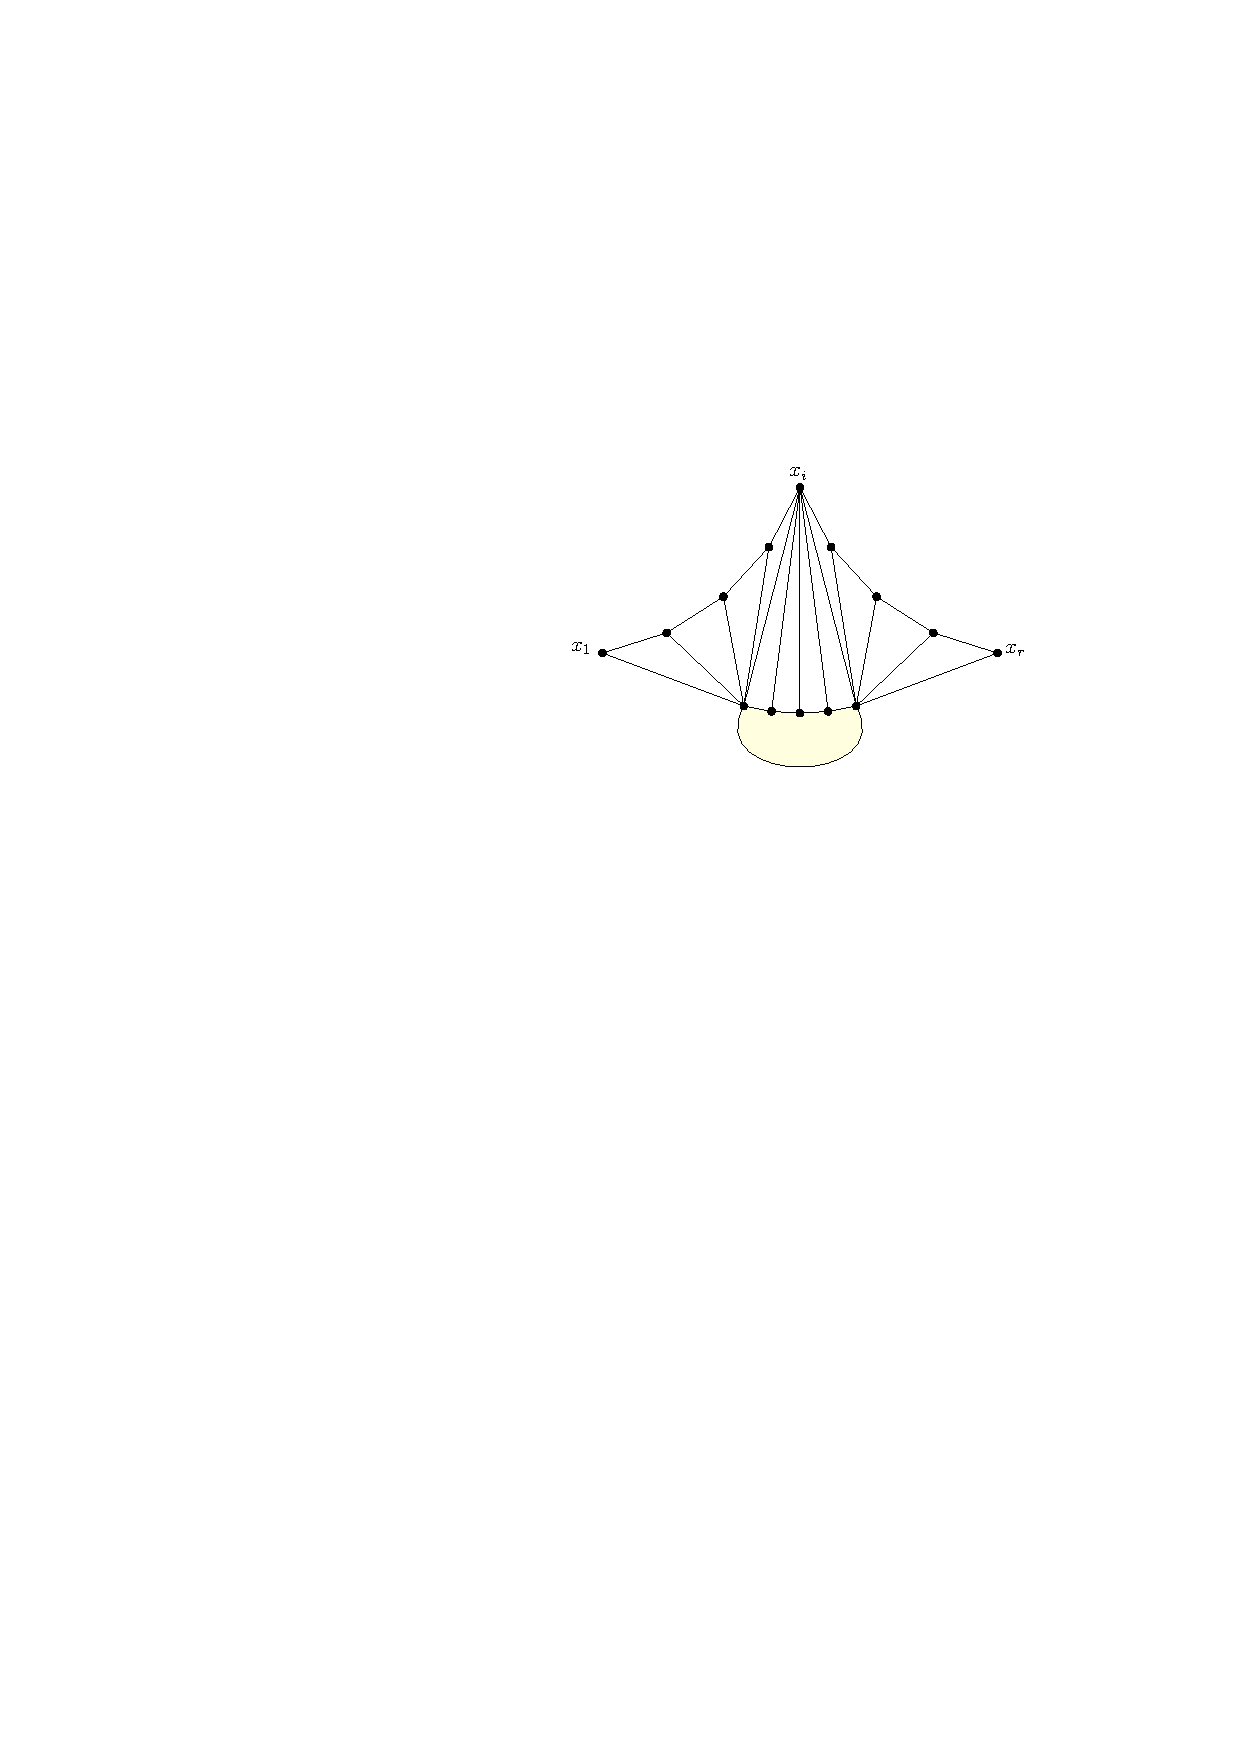
\includegraphics{figs/stingray}
  \end{center}
  \caption{A stingray $x_1,\ldots,x_r$ with stinger $x_i$}
  \label{crow}
\end{figure}

The proof of the following lemma appears in, for example [CITATION],

\begin{lem}\label{crow_proof}
  For any near-triangulation $G$ and any edge $v_1v_2$ on the outer face of $G$, $G$ has a stingray $x_1,\ldots,x_r$ that does not include $v_0$ or $v_1$.
\end{lem}

\begin{proof}
  TODO
\end{proof}

For a triangulation $G$ and an edge $v_1v_2$ on the outer face of $G$, a $v_1v_2$-rooted \defin{stingray decomposition} $S_0,S_1,\ldots,S_t$ is a partition of $V(G)$ such that, $|S_0|=3$, $v_1,v_2\in S_0$ and, for each $i\in\{1,\ldots,t\}$, $S_i$ is a stingray in the near-triangulation $G[\bigcup_{j=1}^{i} S_j]$.  The existence of a stingray decomposition for a triangulation $G$ follows immediately from repeated applications of \cref{crow_proof}.

For a stingray $S:=x_1,\ldots,x_r$ with stinger $x_i$, define the vertex sequence
\[
   \widehat{S} =
   x_i,\quad
   x_{i-1},\ldots,x_{1},\quad
   x_{i+1},\ldots,x_r
\]
For the first set $S_0$ in a $v_1v_2$-rooted stingray decomposition, let $\widehat{S}_0:=v_1,v_2,v_3$ where $v_3$ is the third vertex in $S_0$.
A $v_1v_2$-rooted stingray decomposition $S_0,\ldots,S_t$ of $G$ gives a canonical ordering of $G$, called a \defin{stingray ordering}, defined as the concatenation of $\widehat{S}_0,\widehat{S}_1,\ldots,\widehat{S}_t$.
%
% defined as follows:
% \begin{compactenum}
%   \item The ordering begins with vertices $v_1,v_2,v_3$, where $v_3$ is the third vertex in the graph If $G$ has only three vertices $v_1,v_2,v_3$ then $v_1,v_2,v_3$ is the stingray order.
%   \item If $G$ has $n\ge 4$ vertices then, by \cref{crow_proof} $G$ contains a stingray $x_1,\ldots,x_r$ with stinger $x_i$ that avoids $v_1$ and $v_2$.  Inductively compute a stingray ordering $v_1,v_2,\ldots,v_{n-r}$ for the near-triangulation $G-\{x_1,\ldots,x_r\}$ and make the stingray ordering
%   \[
%     v_1,v_2,\ldots,v_{n-r},\quad
%     x_i,\quad
%     x_{i-1},\ldots,x_{1},\quad
%     x_{i+1},\ldots,x_r
%   \]
% \end{compactenum}

\subsection{Canonical Orderings and Frames}

Any canonical ordering $v_1,\ldots,v_n$ of a triangulation $G$ defines a sequence of graphs $G_2,\ldots,G_n$, where $G_i:=G[v_1,\ldots,v_i]$.  Each of these graphs has the edge $v_1v_2$ on its outer face.  For each $i\ge 2$, each graph $G_i$ contains two edges $u_iv_i$ and $v_iw_i$ incident to $v_i$.   The \defin{frame graph} $F_i$ is the graph with vertex set $V(F_i):=\{v_1,\ldots,v_i\}$ and edge set $E(F_i):=\{v_1v_2\}\cup \bigcup_{j=3}^i\{u_iv_i,v_iw_i\}$.  We treat each frame graph $F_i$ as a directed acyclic graph with the edges directed so that $F_i$ has a single source $v_1$ and a single sink $v_2$ and the orientation of each edge other and $u_iv_i$ and $v_iw_i$ is inherited from $F_{i-1}$.

\subsection{\boldmath Embedding into $U_{n,r,c}$}

To embed an $n$-vertex triangulation $G$ into $U_{n,r,c}$, we start with a $v_1v_2$-rooted stingray decomposition $S_0,\ldots,S_t$ of $G$ and the resulting stingray ordering $v_1,\ldots,v_n$.  For each $j\in\{1,\ldots,t\}$, all the vertices in $S_j$ will be mapped to vertices in the $j$-th row $R_j:=\{x_{i,j}:i\in\{1,\ldots,2^{r+1}-1\}\}$ of $U_{n,r,c}$.  This determines the y-coordinate of each vertex of $G$.

The (directed acyclic) frame graph $F_n$ defines a partial order $\prec$ on the vertices of $G$ in which $v\prec w$ if and only if $F_n$ contains a directed path from $v$ to $w$.  We classify each edge of $F_n$ as \defin{solid} or \defin{vanishing} as follows:  An edge $uw$ of $F_n$ is if there exists some $j\in\{i+1,\ldots,n\}$ such that $u_j=u$ and $w_j=w$; otherwise $uw$ is solid.  Observe that $v_1v_2$ is solid because $u_n=v_1$ and $w_n=v_2$.  For a solid edge $\overrightarrow{uw}$ of $F_n$, define \defin{subdistance} $\sd(u,w)$ from $u$ to $w$ as the maximum number of solid edges in a directed path from $u$ to $w$ in $F_n$.  For a vanish edge $uw$, define $\sd(uw):=0$.

% We use the term subdistance because for any $u\prec v\prec w$, $\sd(u,v)+\sd(v,w) \le \sd(u,w)$.  That is, subdistance satisfies a reverse triangle inequality with equality if and only if there is a longest directed path from $u$ to $w$ that includes $v$.  It is worth noting that in the following paragraphs $\sd(v,w)$ always refers to the length of the longest directed path from $v$ to $w$ in the frame $F_n$, even when we are discussing the frame $F_i$ for some $i<n$.

\paragraph{Subdistances and edge lengths}

Our strategy now is to assign edge ``lengths'' to the edges of $F_n$ so that, for any $u\prec w$, all directed paths from $u$ to $w$ have the same length.  More precisely, we will assign a value $\len(vw)\ge\sd(v,w)$ to each directed edge $\overrightarrow{vw}$ of $F_n$.  For any vertex pair $x\prec y$ in $F_n$ and any directed path $P$ from $x$ to $y$ in $F_n$, this defines $\len(P):=\sum_{e\in E(P)}\len(e)$.  Our assignment will guarantee that for any any vertex pair $x\prec y$ in $F_n$ and any two directed path $P_1$ and $P_2$ from $x$ to $y$ in $F_n$, $\len(P_1)=\len(P_2)$.

We assign these edge lengths in the order edges appear in the sequence $F_2,\ldots,F_n$ of frame graphs.  The root edge $v_1v_2$ is assigned the length $\len(v_1v_2):=\sd(v_1,v_2)$. Now suppose that $\len(vw)$ has been assigned to each directed edge $\overrightarrow{vw}$ in $F_{i-1}$ in such a way that for each vertex pair $v\prec w$ in $F_{i-1}$ and any two directed paths $P_1$ and $P_2$ from $v$ to $w$ in $F_{i-1}$, $\sum_{e\in E(P_1)}\len(e) = \sum_{e\in E(P_2)}\len(e)=:\len(v,w)$.  Next, consider the two directed edges $\overrightarrow{u_iv_i}$ and $\overrightarrow{v_iw_i}$ that appear in $F_i$. If $\sd(u_i,v_i)+\sd(v_i,w_i)=\len(u_i,w_i)$ then we set $\len(u_iv_i):=\sd(u_i,v_i)$ and $\len(v_iw_i):=\sd(v_i,w_i)$.  Otherwise, our action depends on the role of $v_i$ in the stingray $S_k$ that contains $v_i$.  Suppose that $S_k:=x_1,\ldots,x_r$ has stinger $x_j$.  There are three cases to consider.  The handling of the first two is critical for the analysis we will perform later.
\begin{compactenum}
  \item If $v_i=x_j+1$ then $u_i=x_j$ and $\overrightarrow{u_iw_i}$ is an edge of $F_{i-1}$.  In this case we set $\len(u_iv_i):=\len(u_iw_i)-\sd(v_i,w_i)$ and $\len(v_iw_i):=\sd(v_i,w_i)$.

  \item If $v_i=x_{j-1}$ then $w_i=x_j$ and $\overrightarrow{u_iw_i}$ is an edge of $F_{i-1}$.  In this case set $\len(u_iv_i):=\sd(u_i,v_i)$ and $\len(v_iw_i):=\len(u_iw_i)-\sd(v_i,w_i)$.

  \item Otherwise $v_i=x_p$ for some $p\in\{1,\ldots,r\}\setminus\{j-1,j+1\}$. How this is resolved is less important and we can assign $\len(u_iv_i)$ and $\len(v_iw_i)$ using anything that satisfies $\len(u_iv_i)\ge\sd(u_i,v_i)$, $\len(v_iw_i)\ge\sd(v_i,w_i)$ and $\len(u_iv_i)+\len(v_iw_i)=\len(u_iw_i)$.  For example, setting $\Delta_i:=\len(u_i,w_i)-\sd(u_i,v_i)-\sd(v_i,w_i)$,  $\len(u_iv_i):=\sd(u_i,v_i)+\Delta_i/2$, and $\len(v_iw_i):=\sd(v_i,w_i)+\Delta_i/2$ works.
\end{compactenum}
Now consider some vertex pair $v\prec w$ in $F_i$ and some directed path $P$ from $v$ to $w$ in $F_i$.  If $v_i$ appears as in internal vertex in $P$, then removing $v_i$ produces a directed path $P'$ in $F_{i-1}$ with $\len(P)=\len(P')$. .... SAY MORE

\paragraph{Vertex weights}

Ultimately, we want to define a map $\varphi:V(G)\to V(U_{n,r,c})$ so that edges of $G$ are mapped to pairwise non-crossing edges of $U_{n,r,c}$.  This introduces two conflicting requirements. To ensure that edges are pairwise non-crossing we will ensure that for any directed edge $\overrightarrow{vw}$ of $F_n$, $\phi(v)$ has a smaller x-coordinate than $\phi(w)$.   However, we must also ensure that the edge between $\phi(v)$ and $\phi(w)$ appears in $U_{n,r,c}$. This requires that we map at least one of $v$ or $w$ to a value in the majorization sequence that is larger than the difference in x-coordinates between $\phi(v)$ and $\phi(w)$.

To do this we will first assign a weight $\sigma$ to each vertex $v$ of $G$ and require that the x-coordinate $x(v)$ be such that $s_{r,x(v)} \ge \sigma(v)$.  We now describe the process of assigning these weights.

We start by assigning each vertex $v_i$ a \defin{down weight} $\sigma_1(v_i)$. The first two vertices $v_1$ and $v_2$ are special, and have $\sigma(v_1):=\sigma(v_2):=0$.  For $i\ge 2$ the down weight assigned to $v_i$ depends on the role $v_i$ plays in the stingray $S_k$ that contains $v_i$.  Otherwise, our action depends on the role of $v_i$ in the stingray $S_k$ that contains $v_i$.  Suppose that $S_k:=x_1,\ldots,x_r$ has stinger $x_j$.  There are two cases to consider.
\begin{compactenum}
  \item If $v_i\in\{x_1,x_j,x_p\}$ then we set $\sigma_1(v_i):=\len(u_i,w_i)$.

  \item Otherwise $v_i=x_p$ for some $p\in\{1,\ldots,r\}\setminus\{x_1,x_j,x_p\}$ and we set $\sigma_1(v_i):=\len(x_{p-1},x_{p+1})$.
\end{compactenum}

Consider some directed path $P:=z_1,\ldots,z_\ell$ from $v_1$ to $v_2$ in $F_n$.  A \defin{segment} of $P$ is a maximal subpath $z_i,\ldots,z_j$ such that all edges in the subpath are vanishing.  (Note that a segment consists of a single vertex $z_i$ when $z_{i-1}$ and $z_{i+1}$ are both solid.) The \defin{down weight} of a segment $z_i,\ldots,z_j$ is equal to $\max\{\sigma_1(z_p):p\in\{i,\ldots,j\}\}$.  The \defin{down weight} $\sigma_1(P)$ of $P$ is equal to the sum of the down weights of the segments in $P$.



\begin{lem}
  For any directed path $P$ from $v_1$ to $v_2$ in $F_n$, $\sum_{v\in V(P)} \sigma_1(v) \le Cn$.
\end{lem}

\begin{proof}
  By definition, $\len(P)=\len(v_1v_2)$ is the number of edges in the longest directed path in $F_n$ from $v_1$ to $v_2$, so $\len(P)\le n$.
\end{proof}



\end{document}
